\documentclass[12pt,a4paper]{report}
\usepackage{graphicx}
\usepackage{pifont}
\usepackage{dblfnote}
\usepackage{scrextend}
\usepackage{listings}
\DFNalwaysdouble % for this example
\usepackage[Kashida]{xepersian}
\usepackage{xepersian-mathdigitspec}



%\usepackage{xepersian-hm}
\KashidaOn
%\settextfont{B nazanin.TTF}
\settextfont{Vazir.ttf}
\title{طراحی کنترل پیش بین برمبنای یادگیری تقویتی در سامانه تعقیب مسیر خودرو خودران}
\author{\large{سید محمد امین سادات}\\ \\ 
	دانشگاه شهید بهشتی\\ \\
	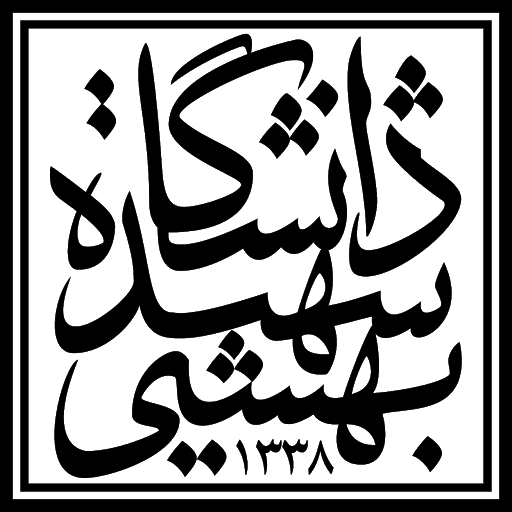
\includegraphics[width = 0.3\linewidth]{logo.jpg}	\\ \\ \\ \\
	استاد راهنما اول :\\ دکتر مصطفی تقی زاده\\ \\
	استاد راهنما دوم :\\ دکتر هادی اشعریون\\ \\
	استاد مشاور      :\\ دکتر محمود مزارع
}
\date{}

\begin{document}
	\maketitle
	\pagebreak
	\tableofcontents
	\pagebreak
	\listoffigures
	\pagebreak
	\begin{abstract}
		یکی از موضوعات مهم در خودرو خودران\footnote{\lr{autonomous vehicle}}، طراحی مسیر\footnote{\lr{path planning}} و تعقیب مسیر\footnote{\lr{path tracking}} است.روش های متفاوتی برای این موضوع ارائه شده است، روش هایی از طریق کاملا با استفاده از هوش مصنوعی تا روش های کاملا مبتی بر دانش کنترل. در این گزارش سعی شده تا یک دیدگاه کلی درباره این موضوع و روش های ارائه شده و روش هایی که قابل استفاده هستند داده شود. 
	\end{abstract}
	
	
	
	\chapter{مقدمه}
	\section{کنترل پیش بین}
	
	
	کنترل پیش بین \footnote{\lr{Model Predictive Control (MPC)}} ریشه در مهندسی کنترل اتوماتیک و بهنیه سازی دارد. در طی دهه های گذشته این روش ارتقا یافته است. بخشی از تاریخچه این علم در اینجا آورده شده است.\\
	\textbf{دهه 60 و 70 میلادی:}
	
	
	در طی این دو دهه اولین جرقه های کنترل پیش بین زده شد. با استفاده از مفاهیم کنترل بهینه که در آن فرمان کنترلی محاسبه میشود که در آن ویژگی ها مد نظر بهینه میشود در این دوره انجام شد. محققان شروع به استفاده از مفاهیم بهینه سازی در حل مسائل کنترل کردند.\\
	\textbf{دهه 80 میلادی:}
	
	
	در طی این دهه ایده های اولیه کنترل پیش بین شکل گرفت. محققان دریافتند که با فرمول کردن معادلات ریاضی سیستم و پیش بینی کردن رفتار آینده سیستم و استفاده از الگوریتم های بهینه سازی برای پیدا کردن فرمان کنترلی که تابع هدف در در یک افق مدت زمان محدود پیدا کرد.\\
	یکی از بزرگترین پیشترفت ها طی این دوره، کشف الگوریتم ماتریس دینامکی کنترل\footnote{\lr{Dynamic Matrix Control (DMC)}} بود. این الگوریتم یک روش کاربردی برای پیاده سازی کنترل پیش بین و ایده استفاده از افق تخمین بود.\\
	\textbf{دهه 90 میلادی:}
	
	در این دهه یک جهش بزرگ در زمینه کنترل پیش بین رخ داد. محققان الگوریتم های پیچیده تر کشف کردند که باعث ارتقای عملکرد و پیاده سازی کنترل پیش بین شد.\\
	یکی از پیشرفت هایی که در دوره اتفاق افتاد معرفی کنترل پیش بین غیر خطی \footnote{\lr{Non-linear MPC}}بود که میتوانست سیستم هایی با دینامیک غیر خطی را پوشش دهد. روش هایی نظیر خطی سازی و بهینه سازی استفاده شدند تا مدل غیر خطی را تخمین بزنند و مسئله را بصورت مکرر\footnote{\lr{iterative}} حل کنند.\\
	\textbf{دهه اول 2000:}
	
	در طی این زمان کنترل پیش بین بصورت گسترده در صنعت استفاده می شد. وجود منابع محاسباتی قوی و پیشرفت الگوریتم های بهینه سازی زمینه استفاده و پیاده سازی کنرل پیش بین را فراهم کرده بود.\\
	محققان بهبود بخشیدن به کنترل پیش بین را ادامه دادند و باعث کشف افزونه های جدید کنترل پیش بین مانند:
	\begin{itemize}
		\item[\ding{70}]  کنترل پیش بین مقاوم\footnote{\lr{robust MPC}}\cite{campo1987robust}
		\item[\ding{70}]   کنترل پیش بین تصادفی\footnote{\lr{stochastic MPC}}
		\item[\ding{70}]  کنترل پیش بین اقتصادی\footnote{\lr{economic MPC}} 
	\end{itemize}
	که هر کدام مسئله خاصی را میتوااند حل کنند و عدم قطعیت در سیستم است.\\
	\textbf{دهه دوم 2000 تا حال:}
	
	در سال های اخیر کنترل پیش بین ارتقا یافته است و در زمینه های مختلفی استفاده میشود. پیشرفت یادگیری ماشین و روش های داده محور محققان توانستند این روش ها را با کنترل پیش بین ترکیب کنند. علاوه بر این کتابخانه ها و نرم افزار هایی در جهت استفاده راحت تر کاربر وارد بازار شده است.\\
	امروزه کنترل پیش بین در زمینه هاو صنعت هایی مانند: کنترل پروسه های شیمیایی، سیستم های قدرت، رباتیک، ماشین های خودران و \lr{\dots} استفاده میشود. نقاط قوت کنترل پیش بین در بهینه سازی سیستماتیک، هندل کردن قیود سیستم و تطبیق پذیری به مسائل پیچیده کنترلی است که باعث شده کنترل پیش بین یک روش ارزشمند در خیلی از مسائل روزمره باشد.
	
	\section{یادگیری تقویتی}
	یادگیری تقویتی \footnote{\lr{Reinforcement Learning (RL)}} شاخه ای از علم یادگیری ماشین است که تمرکز دارد به یافتن الگوریتم و روش هایی که یک عامل \footnote{\lr{Agent}} رفتار بهینه را از طریق تعامل با محیط\footnote{\lr{environment}} یاد میگیرد. \\
	\textbf{دهه 50 و 60 میلادی:}
	
	منشأ یادگیری تقویتی به دهه 50 و تحقیقات ریچار بلمن\footnote{\lr{Richard Bellman}} در موضوع برنامه نویسی پویا\footnote{\lr{dynamic programming}} \cite{Bellman:DynamicProgramming} برمیگردد. معادلات بلمن یک اساس تئوری برای حل کردن مسائل کنترل بهینه در یک محیط با عدم قطعیت را فراهم میسازد. این معادلات مقدمات یادگیری تقویتی را فراهم میسازد.\\
	\textbf{دهه 70 و 80 میلادی:}
	
	در این دو دهه پیشرفت قابل توجهی در یادگیری تقویتی صورت گرفت. یکی از این زحمات توسعه الگوریتم تفاوت زمانی\footnote{\lr{Temporal Diffrence (TD)}} به وسیله ریچارد ساتون\footnote{\lr{Richard Sutton}} است. الگوریتم یادگیری تفاوت زمانی مفهوم \cite{sutton1988learning}به روز کردن تخمین ارزش\footnote{\lr{value}} بر مبنای اختلاف بین پاداش\footnote{\lr{reward}} تخمین زده و مشاهده شده را معرفی کرد.\\
	نقطه عطف دیگر، معرفی الگوریتم یاگیری کیو \footnote{\lr{Q-learning}} توسط کریستوفر واتکینز\footnote{\lr{Christopher Watkins}} \cite{watkins1992q}در سال 1989 است. یادگیری کیو یک روش بدون مدل است تابع عمل-ارزش\footnote{\lr{action-value}} را یاد میگیرد و این الگوریتم بصورت گسترده در مسائل یادگیری تقویتی استفاده میشود.\\
	\textbf{دهه 90 و اوایل 2000:}
	
	
	در طی این دوره الگوریتم های پیچیده یاگیری تقویتی توسعه پیدا کردند. یکی از این پیشرفت ها معرفی الگوریتم های گرادیان سیاست\footnote{\lr{policy gradient}} است که در آن سیاست بطور مستقیم بهینه میشود در مقابل روش های قبلی که تابع ارزش تخمین زده میشد. روش هایی مثل تقویت\footnote{\lr{REINFORCE}} که توسط رونالد ویلیامز\footnote{\lr{Ronald J. Williams}} در سال 1992 و بازیگر-منتقد\footnote{\lr{actor-critic}} در طی این زمان محبوبیت زیادی پیدا کردند.\\
	\textbf{اواخر 2000و2010:}
	
	در طی این سال ها هم یادگیری تقویتی پیشرفت سریعی داشت، که بخاطر افزایش سرعت محاسبات  و پیشرفت یادگیری عمیق\footnote{\lr{deep learning}} بود. یاگیری عمیق تقویتی\footnote{\lr{deep reinforcement learning}} به عنوان یک روش قوی که شبکه عصبی مصنوعی\footnote{\lr{neural networks}} را با الگوریتم های یادگیری تقویتی ترکیب میکرد ظهور کرد.\\
	یک پیشرفت بزرگ در سال 2013 معرفی الگوریتم یادگیری عمیق کیو\footnote{\lr{Deep Q-learning  (DQN)}} \cite{mnih2015human} توسط ولادیمیر منیه\footnote{\lr{Voldymyr Mnih}} است. این الگوریتم در بازی های آتاری که فقط به عنوان ورودی پیکسل های عکس را دریافت میکرد عملکرد خیره کننده به جا گذاشت.\\
	سال های بعد هم موفقیت های زیادی در این زمینه اتفاق افتاد مثل توسعه الگوریتم های بهبنه سازی سیاست نزدیک\footnote{\lr{proximal policy optimization (PPO)}} \cite{schulman2017proximal}و بهینه سازی سیاست منطقه اعتماد\footnote{\lr{trust region policy optimization (TRPO)}} \cite{schulman2015trust}و بازیگر-منقد مزیت ناهمگام\footnote{\lr{asynchronous advantage actor-critic (A3C)}} \cite{mnih2016asynchronous}.\\	
	\textbf{حال حاظر:}

در حال حاظر نیز محققان در حال تحقیق و توسعه الگوریتم های جدید و پیاده سازی آن ها روی مسائل روزمره مانند رباتیک، بهداشت، مسائل مالی و سیستم های خودران. در حال حاظر بیشتر تمرکز روی بهبود بخشیدن مشکلات یاگیری تقویتی است مثل بازده پایین، امنیت و توانایی حل کردن مسائل بزرگ و مسائل کنترلی پیوسته است.	
	\section{خودرو خودران}
	پیشینه خودرو خودران\footnote{\lr{autonomous vehicle}} به خودرو های ار سی بر میگردد. محققان به دنبال راهی بودند که خودرو بدون دخالت انسان حرکت کند.\\
	دهه 60 و 70 میلادی:
	
	اولین پیشرفت ها در این علم صورت گرفت. سبد خرید استفورد\footnote{\lr{Stanford cart}} که توسط دانشگاه استنفورد در دهه 60 ساخته شده بود. این خودرو از برای موقعیت یابی استفاده میکرد و میتوانست میسر از پیش تعیین شده را دنبال کند.\\
	\textbf{دهه 80 و 90 میلادی:}
	
	در طی این دو دهه پیشرفت های بزرگی صورت گرفت. خودرو \lr{ALV} توسط ارنتست دیکمنز در دانشگاه بندشور مونیخ ساخته شد. این خودرو توانایی درک محیط از طریق سنسور بینایی و برنامه ریزی مسیر بصورت دینامیکی را داشت و بنیان گذار خودرو خودران بود.\\
	سالهای 2000 و 2010:
	
	در سال 2004 مسابقه بزرگ دارپا\footnote{\lr{DARPA}} که توسط وزارت دفاع آمریکا برگزار شد. این مسابقه با هدف ترویج توسعه خودرو های خودران  که توانایی به اتمام رساندن یک مسیر جاده خاکی بیابانی صورت گرفت. در حالی که هیچ خودرویی در مسابقه اول نتوانست مسیر را کامل طی کند اما در مسابقه های بعدی که در سال های 2005 و 2007 برگزار شد چندین خودرو موفق به پایان ساندل مسیر شدند.\\
	در طی این دوره شرکت های بزگی مثل گوگل و اوبر سرمایه گزاری سنگینی بر روی خودرو های خودران کردند. پروژه خودرو خودران گوگل در سال 2009 شروع شد، و بر روی توسعه سیستم های ادراکی مقاوم و الگوریتم های یاگیری ماشین برای خودرو های خودران تمرکز داشت.\\
	در سال 2012 ورود این خودرو ها به خیابان های ایالت نوادا آمریکا قانونی شد و گام بزرگی در جهت توسعه این خودرو ها برداشته شد.\\
	2010 تا حال:
	
	در اوایل دهه 2010 نقطه عطف قابل توجه برای صنعت خودرو های خودران بود. شرکت های بزگی مثل تسلا، جنرال موتورز، آیودی و ...  شروع به اضافه کردن قابلیت های نمیه خودران به خط تولید خودرو های خود کردند.\\
	پیشرفت در تکنولوژی سنسوری، یادگیری ماشین و هوش مصنوعی باعث پیشرفت بیشتر در این خورو ها گردید. سنسور هایی نظیر لیدار\footnote{\lr{Light Detection and Ranging (LiDAR)}}، رادار\footnote{\lr{radar}}، و دوربین به عضو جدا ناپذیر این خودرو ها تبدیل شدند. الگوریتم های پیچیده برای درک، محلی سازی\footnote{\lr{localization}}، نقشه برداری\footnote{\lr{mapping}}، و تصمیم گیری توسعه یافت.\\
	توسعه چارچوب های نظارتی و استاندارد صنعتی در طی سال های اخیر مورد توجه قرار گرفته است. دولت ها و شرکت ها در سطح جهان در کنار هم کار میکنند تا دستورالعمل های جهانی برای تست و گسترش این خودرو ها انجام دهند.\\
	در حال حاظر زمینه خودرو های خودران رشد بسیار سریعی داشته. تحقیق و توسعه زیادی در حال حاظر در جهت پیشبرد امنیت، اطمینان، مقیاس پذیری در حال انجام است. ورود خودرو های تمام خودران به خیابان های عمومی هنوز هم چالش بزرگی است. این چالش نیازمند پیشرفت در تکنولوژی، زیرساخت و مقررات است.
	\section{طرح چالش}
	یکی از چالش های بزرگ در خودرو های خودران مسئله طراحی مسیر و تعقیب مسیر تأیین شده توسط خودرو است. این مسئله به طور مستقیم به جان انسان ها مرتبط است، اگر خطایی در سیستم به وجود بیاید ممکن است اثار جبران نا پذیری را روی زنگی افراد بگزاد. این سیستم باید بتواند خطرات مختلف مثل سرعت خودرو های اطراف، عابران پیاده، انحنای مسیر، سرعت های مختلف، راحتی سرنشینان خودرو و ...   را در نظر بگیرد. الگوریتم های زیادی برای حل این موضوع استفاده شده است هر کدام با دقت ها و پیچیدگی های متفاوت. به نظر میرسد که به دلیل اهمیت بالای مسئله و اینکه به طور مستقیم به زندگی افراد ربط دارد بهتر است سادگی فدای دقت شود تا از حوادث ناگوار بهتر بتوان پیشگیری کرد. امروزه با پیشرفت رایانه ها و سرعت های محاسباتی قابل توجه شان میتوان الگوریتم های پیچیده را به راحتی پیاده سازی کرد. \\
	\begin{figure}
		\centering
		\includegraphics[width=\linewidth]{figs/8.jpg}
		\caption{ کنترل کننده برمبنای یادگیری تقویتی}
		\label{fig:intro}
	\end{figure}
	همانطور که در شکل \ref{fig:intro} میبینید، یک ساختار کلی کنترل کننده یادگیری تقویتی برای سیستم تعقیب میسر خودرو است. در این شکل یک طرح کلی از ساختار کنترلی مشاهده میشود.
	\chapter{پیشینه تحقیقات}
	در مقاله \cite{alhazmi2022reinforcement} یک روش خلاقانه در ترکیب کنترل پیش بین غیر خطی و یادگیری تویتی صورت گرفته است. در این مقاله با استفاده از الگوریتم \lr{DDPG}\cite{lillicrap2015continuous} پارامتر های مدل تخمین زده میشود و با استفاده از این پارامتر های تخمین زده شده و حالت های اندازه گیری شده از محیط بقیه حالت های غیر قابل اندازه گیری تخمین زده میشوند و سپس این مقدایر تخمین زده شده به کنترل کننده اصلی که کنترل پیش بین است داده می شود تا فرمان کنترلی خود را تولید کند. این کنترل کننده بر روی سیستم تانک تست شده است.
	\begin{figure}
		\includegraphics[width=\linewidth]{figs/1.jpg}
		\caption{ساختار کنترلی مقاله \cite{alhazmi2022reinforcement}}
		\label{fig:DDPG_MPC}
	\end{figure}

	\begin{figure}
		\includegraphics[width=\linewidth]{figs/2.jpg}
		\caption{پاسخ های مقاله \cite{alhazmi2022reinforcement}}
		\label{fig:DDPG_MPC_RES}
	\end{figure}
	در شکل \ref{fig:DDPG_MPC} ساختار کنترلی پیشنهادی این مقاله و نحوه ترکیب کنترل پیش بین غیر خطی با الگوریتم  \lr{DDPG} مشاهده میکنید. در شکل \ref{fig:DDPG_MPC_RES} پاسخ های سیستم را مشاهده میکنید؛ چهار نمودار سمت چپ پاسخ سیستم بدون حضور اغتشاش را نشان میدهد و چهار نمودار سمت راست نیز پاسخ سیستم  در حضور اغتشاش را نشان میدهد. همانطور که در شکل مشخص است پاسخ های سیستم بسیار به میزان معیار خود نزدیک هستند.\\
	
	
	در مقاله \cite{zhang2022robust} یک روش خلاقانه دیگر استفاده شده، در این مقاله ابتدا با استفاده از اپراتور کوپمن\footnote{\lr{Koopman operator}} سیستم معالات به بک فضای بینهاین هیلبرت\footnote{\lr{hilbert space}} برده میشود، سپس با استفاده از این تغییر معادلات سیستم بدون اینکه محدود به یک بازه تغییراتی خاص باشند، خطی میشوند. در این مقاله ابتدا مغتیر های حالت اندازه گیری شده ابتدا به فضای هیلبرتی برده می شوند، سپس خطای بین مقدار اندازه گیری شده در شبکه منتقد\footnote{\lr{critic network}} و مقدار واقعی اندازه گیری میشود و در یک ضریب افزایشی ضرب\footnote{\lr{gain}} میشود و قسمت اول فرمان کنترلی صادر میشود. قسمت دوم فرمان کنترلی با استفاده از مدل و شبکه بازیگر\footnote{\lr{actor network}} ساخته میشود. این کنترل کننده بر روی سیستم پاندول-واگن پیاده سازی شده است در شکل \ref{fig:KMPC} ساختار کنترلی پیشنهادی این مقاله را مشاهده میکنید. پاسخ های این سیستم همانطور که در شکل \ref{fig:KMPC_res} مشخص است هم به مقدار معیار خود بسیار نزدیک و در کل عملکرد بسیار عالی داشته است.\\
	\begin{figure}
		\includegraphics[width=\linewidth]{figs/12.jpg}
		\caption{ساختار کنترلی در مقاله \cite{zhang2022robust}}
		\label{fig:KMPC}
	\end{figure}
	\begin{figure}
		\includegraphics[width=\linewidth]{figs/13.jpg}
		\caption{پاسخ های سیستم در مقاله \cite{zhang2022robust}}
		\label{fig:KMPC_res}
	\end{figure}
	
	در مقاله \cite{wang2022data} برای کنترل کننده، یک کنترل کننده پیش بین بر مبنای اپراتور کوپمن پیشنهاد شده که وظیفه تعقب مسیر را دارد، است. این کنترل پیشنهادی برای تبدیل کردن سیستم غیر خطی به سیستم خطی از یک شبکه عصبی برای رمزنگاری و رمزگشایی استفاده میکند. که ساختار مورد استفاده را در شکل \ref{fig:data} مشاهده می کنید. این کنترل کننده میتواند بدون دانستن دینامیک سیستم عمل کند. تست این کنترل کننده بر روی یک ربات انجام شده است. در شکل \ref{fig:data_path} مسیر های استفاده شده جهت تست ربات را نشان میدهد و در شکل   \ref{fig:data_res} میزان خطا ها در شکل سمت راست در بین سه شکل\ref{fig:data_path} . \\
	\begin{figure}
		\includegraphics[width=\linewidth]{figs/3.jpg}
		\caption{ساختار کنترلی مقاله\cite{wang2022data}}
		\label{fig:data}
	\end{figure}
	\begin{figure}
		\includegraphics[width=\linewidth]{figs/4.jpg}
		\caption{مسیر های تست مقاله \cite{wang2022data}}
		\label{fig:data_path}
	\end{figure}
	\begin{figure}
		\includegraphics[width=\linewidth]{figs/5.jpg}
		\caption{خطا مسیر}
		\label{fig:data_res}
	\end{figure}
	
	در مقاله \cite{tang2020improved} برای تعقیب مسیر یک روش با استفاده از ترکیب کنترل پیش بین و کنترل \lr{PID} استفاده کرده است. در این مقاله خروجی کنترل کننده پیش بین یک مرجع برای کنترل کننده \lr{PID} است. کنترل کننده \lr{PID} سپس با استفاده از مقدار اندازه گیری شده خطا خودرو را کنترل میکند. کنترل \lr{PID} در اصل مقدار زاویه \lr{yaw} را کنترل مینکد و کنترل پیش بین مقدار سرعت \lr{yaw} را کنترل میکند. در این مقاله برای خودرو از مدل دینامیکی دوچرخه استفاده شده است. در شکل \ref{fig:fuzzy_pid} ساخنتار پیشنهادی این مقاله را مشاهده میکنید.\\
	\begin{figure}
		\includegraphics[width=\linewidth]{figs/6.jpg}
		\caption{ساختار کنترلی مقاله \cite{tang2020improved}}
		\label{fig:fuzzy_pid}
	\end{figure}
	
	در مقاله \cite{wang2019path} برای تعقیب مسیر یک روش دیگر پیشنهاد شده. در این مقاله تعقیب مسیر به صورت اصلی با کنترل کننده پیش بین است، در کنار این کنترل کننده یک کنترل کننده فازی تطبیق پذیر استفاده شده. کنترل کننده فازی نقش پیدا کردن مقادیر بهینه ضرایب کنترل کننده پیش بین را بر عهده دارد، سپس کنترل کننده پیش بین فرمان کنترلی خود را بر اساس ضرایب بهینه تأیین شده را صادر میکند. ساختار کنترلی پیشنهاد شده در این مقاله را در شکل \ref{fig:fuzzy_mpc} مشاهده میکنید.\\
	
	\begin{figure}
		\includegraphics[width=\linewidth]{figs/7.jpg}
		\caption{ساختار کنترلی مقاله \cite{wang2019path}}
		\label{fig:fuzzy_mpc}
	\end{figure}
	
	در مقاله \cite{yao2020control} روش های مختلف برای تعقیب مسیر با هم مقایسه شده. در شکل های \ref{fig:diff1} و \ref{fig:diff2} و \ref{fig:diff3} این مقایسه آمده است. در شکل \ref{fig:diff1} مقایسه بین کنترل کننده و مزیت ها و معایب آن را مشاهده میکنید. در شکل  \ref{fig:diff2} مقایسه بین کنترل کننده های مقاوم و مزایا و معایب آن ها را ماشهده میکنید. و در آخر هم در شکل \ref{fig:diff3} مقایسه بین مشاهده گر های مختلف را مشاهده میکنید.\\
	\begin{figure}
		\includegraphics[width=\linewidth]{figs/9.jpg}
		\caption{مقایسه کنترل کننده های مختلف}
		\label{fig:diff1}
	\end{figure}
	\begin{figure}
		\includegraphics[width=\linewidth]{figs/10.jpg}
		\caption{مقایسه کنترل کننده های مقاوم}
		\label{fig:diff2}
	\end{figure}
	\begin{figure}
		\includegraphics[width=\linewidth]{figs/11.jpg}
		\caption{مقایسه مشاهده گر ها}
		\label{fig:diff3}
	\end{figure}
	
	در مقاله \cite{fang2022auv} برای تعقیب مسیر برای زیر دریایی اتوماتیک یک روش کاملا بر اساس یادگیری تقویتی عمیق پیشنهاد شده. در این روش \lr{DDPG} برای تعقیب مسیر استفاده شده است. ساختار کنترلی پیشنهاد شده را در شکل \ref{fig:auv} می بینید.
	\begin{figure}
		\includegraphics[width=\linewidth]{figs/14.jpg}
		\caption{ساختار کنترلی مقاله \cite{fang2022auv}}
		\label{fig:auv}
	\end{figure}
	
	\chapter{پیشنهادات}
	\section*{استفاده از الگوریتم های دیگر}
	الگوریتم های دیگری در زمینه یادگیری تقویتی وجود دارند که ممکن است در طبق مسئله بهتر جواب دهد. برای مثال:
	\begin{itemize}
		\item[\ding{70}] \lr{DDPG} \footnote{\lr{deep deterministic policy gradient}}
		\item[\ding{70}] \lr{TD3} \footnote{\lr{twin delayed deep determinestic policy gradient}}
		\item[\ding{70}] \lr{SAC} \footnote{\lr{soft actor critic}}
		\item[\ding{70}] \lr{PPO} \footnote{\lr{proximal policy optimization}}
		\item[\ding{70}] \lr{TRPO} \footnote{\lr{trust region policy optimization}}
		\item[\ding{70}] \lr{REINFORCE}
		\item[\ding{70}] \lr{A2C} \footnote{\lr{advantage actor critic}}
	\end{itemize}
	بعضی از این الگوریتم ها ساده تر و برخی پیچیده تر از بقیه هستند که با استفاده از آزمون و خطا میتوان بهترین انتخاب را تشخیص داد.
	\section*{استفاده از تابع هدف اقتصادی}
	به جای استفاده از تابع هدف سهموی\footnote{\lr{quadratic}} از توابع هدف دیگر مثل توابع نمایی استفاده شود.
	\section*{تاخمین زدن اغتشاش}
	میتوان با استفاده از خروجی شبکه تقویتی اغتشاش را در سیستم تخمین زئ و به معادلات کنترل کننده وارد کرد تا نتایج بدست آمده توسط کنترل کننده ضریب اطمینان بالا تری داشته باشد.
	\section*{تخمین زدن معادلات سیستم}
	در بعضی از سیستم ها پارامتر ها با زمان تغییر میکنند. میتوان این تغییر در پارامتر را با استفاده از خروجی شبکه عصبی تخمین زد.
	\section*{استفاده از کنترل های دیگر}
	می توان به جای کنترل کننده پیش بین از کنترل کننده های دیگر مثل:
	\begin{itemize}
		\item[\ding{70}] \lr{PID}
		\item[\ding{70}] \lr{LQR}
		\item[\ding{70}] \lr{Sliding Mode}
		\item[\ding{70}] \lr{Fuzzy}
		\item[\ding{70}] ...
	\end{itemize}
	\section*{امنیت سایبری}
	کنترل کننده ها میتوانند در مقابل خطراتی مثل تزریق داده اشتباه \footnote{\lr{false data injection}} بسیار آسیب پذیر باشند، و در مسائلی مثل خودرو خودران این موضوع بسیار حائز اهمیت است چون به طور مستقیم به امنیت جانی انسان ها هم درون خودرو و هم خارج از خودرو مرتبط است.
	\section*{تشخیص خطا}
	پیدا کردن خطا در سیستم میتواند کمک بسیار بزرگی به تعمیر و رفع مشکل کند. از این رو طراحی سیستم های تشخیص خطا\footnote{\lr{fault detection}} میتواند حائز اهمیت باشد
	\section*{کنترل مقاوم در برابر خطا}
	یکی دیگر از زمینه های مهم کنترل مقاوم در برابر خطا\footnote{\lr{fault telorant control}} است. این طراحی کنترل کننده ای که این ویژگی را داشته باشد میتواند در شرایطی جان سرنشینان یا دیگران را نجات دهد. مثلا در سرعت بالا لاستیک خودرو از سوراخ شود.
	
	
	%\chapter{شبیه سازی اولیه}
	%در این قسمت یک شبیه سازی ساده با استفاده از زبان برنامه نویسی پایتون برای یک خودرو خودران با استفاده از مدل دینامیکی دوچرخه آکرمن انجام شده است. در این شبیه سازی سیستم مقید به تعقیب مسیر خاصی نیست و کنترل کننده تشخیص میدهد که کدام مسیر بهینه ترین مسیر برای خودرو است. کنترل استفاده شده یک کنترل کننده پیش بین غیر خطی است که با استفاده از چارچوب \lr{CasADi} \cite{Andersson2019} و حل کننده \lr{ipopt} \cite{wachter2006implementation} این شبیه سازی انجام شده است. معادله به روش \lr{multiple shooting} گسسته اشت است و به روش \lr{Runge Kuta 4} شبیه سازی شده.
	
	
	\appendix
	%\chapter{کد پایتون}
	%\begin{latin}
	%	\begin{lstlisting}[language=python]
	%		import numpy as np
	%		A = np.zeros(shape = (2,2))
	%	\end{lstlisting}	
	%\end{latin}
	
	
	\bibliographystyle{ieeetr}
	\begin{thebibliography}{10}
		\begin{latin}
			
		
		\bibitem{campo1987robust}
		P.~J. Campo and M.~Morari, ``Robust model predictive control,'' in {\em 1987
			American control conference}, pp.~1021--1026, IEEE, 1987.
		
		\bibitem{Bellman:DynamicProgramming}
		R.~Bellman, {\em {Dynamic Programming}}.
		\newblock Dover Publications, 1957.
		
		\bibitem{sutton1988learning}
		R.~S. Sutton, ``Learning to predict by the methods of temporal differences,''
		{\em Machine learning}, vol.~3, pp.~9--44, 1988.
		
		\bibitem{watkins1992q}
		C.~J. Watkins and P.~Dayan, ``Q-learning,'' {\em Machine learning}, vol.~8,
		pp.~279--292, 1992.
		
		\bibitem{mnih2015human}
		V.~Mnih, K.~Kavukcuoglu, D.~Silver, A.~A. Rusu, J.~Veness, M.~G. Bellemare,
		A.~Graves, M.~Riedmiller, A.~K. Fidjeland, G.~Ostrovski, {\em et~al.},
		``Human-level control through deep reinforcement learning,'' {\em nature},
		vol.~518, no.~7540, pp.~529--533, 2015.
		
		\bibitem{schulman2017proximal}
		J.~Schulman, F.~Wolski, P.~Dhariwal, A.~Radford, and O.~Klimov, ``Proximal
		policy optimization algorithms,'' {\em arXiv preprint arXiv:1707.06347},
		2017.
		
		\bibitem{schulman2015trust}
		J.~Schulman, S.~Levine, P.~Abbeel, M.~Jordan, and P.~Moritz, ``Trust region
		policy optimization,'' in {\em International conference on machine learning},
		pp.~1889--1897, PMLR, 2015.
		
		\bibitem{mnih2016asynchronous}
		V.~Mnih, A.~P. Badia, M.~Mirza, A.~Graves, T.~Lillicrap, T.~Harley, D.~Silver,
		and K.~Kavukcuoglu, ``Asynchronous methods for deep reinforcement learning,''
		in {\em International conference on machine learning}, pp.~1928--1937, PMLR,
		2016.
		
		\bibitem{alhazmi2022reinforcement}
		K.~Alhazmi, F.~Albalawi, and S.~M. Sarathy, ``A reinforcement learning-based
		economic model predictive control framework for autonomous operation of
		chemical reactors,'' {\em Chemical Engineering Journal}, vol.~428, p.~130993,
		2022.
		
		\bibitem{lillicrap2015continuous}
		T.~P. Lillicrap, J.~J. Hunt, A.~Pritzel, N.~Heess, T.~Erez, Y.~Tassa,
		D.~Silver, and D.~Wierstra, ``Continuous control with deep reinforcement
		learning,'' {\em arXiv preprint arXiv:1509.02971}, 2015.
		
		\bibitem{zhang2022robust}
		X.~Zhang, J.~Liu, X.~Xu, S.~Yu, and H.~Chen, ``Robust learning-based predictive
		control for discrete-time nonlinear systems with unknown dynamics and state
		constraints,'' {\em IEEE Transactions on Systems, Man, and Cybernetics:
			Systems}, vol.~52, no.~12, pp.~7314--7327, 2022.
		
		\bibitem{wang2022data}
		Y.~Wang, Y.~Yang, Y.~Pu, and C.~Manzie, ``Data-driven predictive tracking
		control based on koopman operators,'' {\em arXiv preprint arXiv:2208.12000},
		2022.
		
		\bibitem{tang2020improved}
		L.~Tang, F.~Yan, B.~Zou, K.~Wang, and C.~Lv, ``An improved kinematic model
		predictive control for high-speed path tracking of autonomous vehicles,''
		{\em IEEE Access}, vol.~8, pp.~51400--51413, 2020.
		
		\bibitem{wang2019path}
		H.~Wang, B.~Liu, X.~Ping, and Q.~An, ``Path tracking control for autonomous
		vehicles based on an improved mpc,'' {\em IEEE Access}, vol.~7,
		pp.~161064--161073, 2019.
		
		\bibitem{yao2020control}
		Q.~Yao, Y.~Tian, Q.~Wang, and S.~Wang, ``Control strategies on path tracking
		for autonomous vehicle: State of the art and future challenges,'' {\em IEEE
			Access}, vol.~8, pp.~161211--161222, 2020.
		
		\bibitem{fang2022auv}
		Y.~Fang, Z.~Huang, J.~Pu, and J.~Zhang, ``Auv position tracking and trajectory
		control based on fast-deployed deep reinforcement learning method,'' {\em
			Ocean Engineering}, vol.~245, p.~110452, 2022.
		
		\bibitem{Andersson2019}
		J.~A.~E. Andersson, J.~Gillis, G.~Horn, J.~B. Rawlings, and M.~Diehl,
		``{CasADi} -- {A} software framework for nonlinear optimization and optimal
		control,'' {\em Mathematical Programming Computation}, vol.~11, no.~1,
		pp.~1--36, 2019.
		
		\bibitem{wachter2006implementation}
		A.~W{\"a}chter and L.~T. Biegler, ``On the implementation of an interior-point
		filter line-search algorithm for large-scale nonlinear programming,'' {\em
			Mathematical programming}, vol.~106, pp.~25--57, 2006.
		\end{latin}
		
	\end{thebibliography}
	
	
	
\end{document}